%%%%%%%%%%%%%%%%%%%%%%%%%%%%%%%%%%%%%%%%%%%%%%%%%%%%%%%%%%%%%%%%%%%%
\section{Organization}
\label{sec:fdsp-pd-org}
%\metainfo{\color{red}\bf  Content: Segreto/Warner/Mualem}
%\metainfo{(Length: TDR=20 pages, TP=4 pages)}

%%%%%%%%%%%%%%%%%%%%%%%%%%%%%%%%%%%
\subsection{Single-Phase Photon Detection System Consortium Organization}
\label{sec:fdsp-pd-org-consortium}
%\metainfo{\color{blue} Content: Segreto}


The Photon Detection System (PDS) consortium follows the typical organizational structure of DUNE Consortia:
\begin{itemize}
\item A Consortium Lead (Ettore Segreto) provides overall leadership for the effort, and attends meetings of the Executive and Technical Boards.
\item A Technical Lead (David Warner) provides technical support to the consortium lead, attends the Technical Board and Integration/Project meetings, oversees the project schedule and WBS, and oversees the operation of the project working groups.  In the case of the PDS, the Technical Lead is supported by a Deputy Technical Lead (Leon Mualem).
\end{itemize}

\begin{dunefigure}[PDS consortium organization chart.]{fig:pds-org.pdf}
{Photon Detector System consortium organization chart.}
 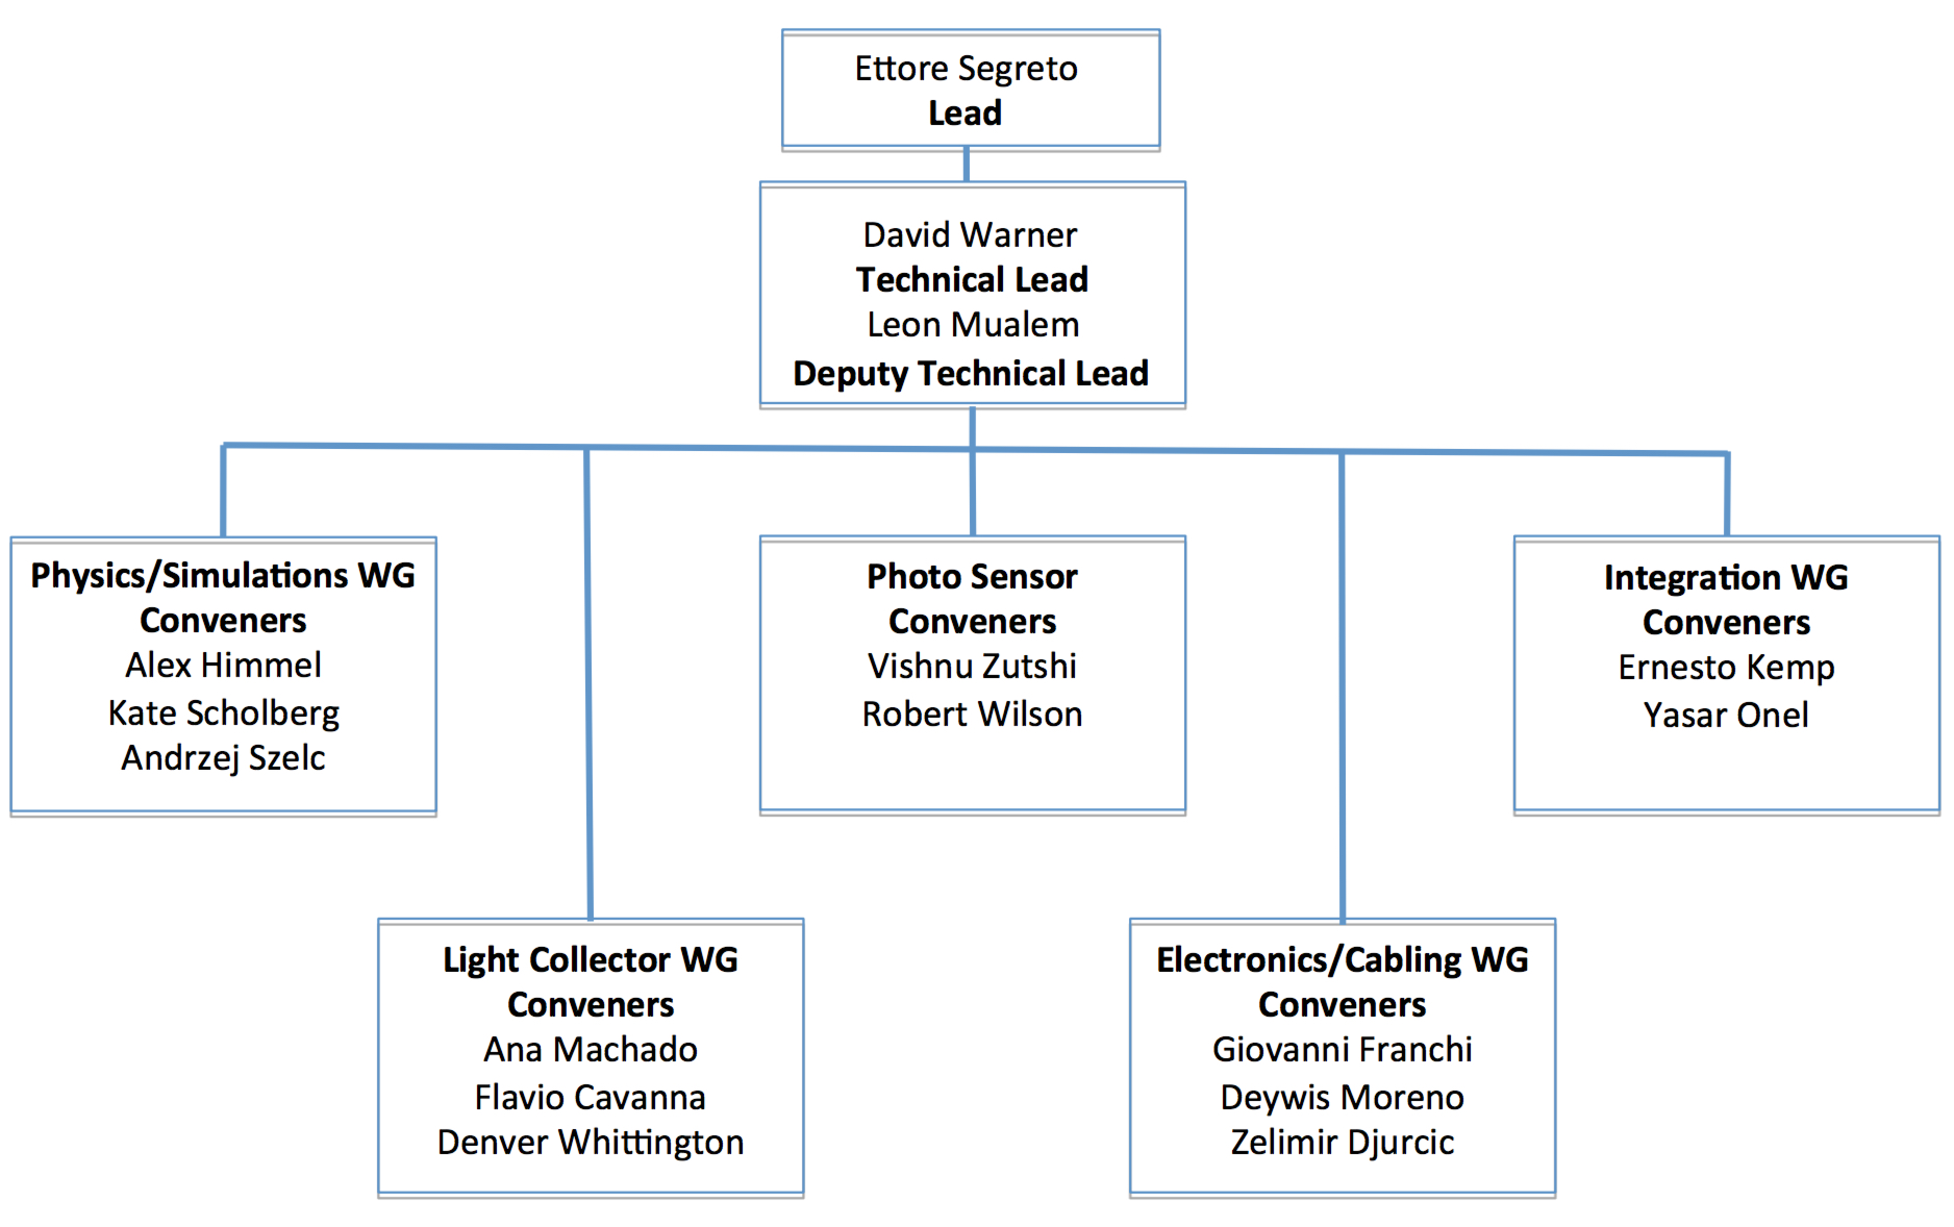
\includegraphics[width=0.8\columnwidth]{pds-org.pdf}
\end{dunefigure}

Below the leadership, the consortium is divided up into five working groups, each led by two or three working group conveners as shown in the PDS Management Table of Organization.  Each working group is charged with one primary area of responsibility within the consortium, and the conveners report directly to the technical lead regarding those responsibilities.  As the consortium advances to a more detailed WBS and project schedule, it is envisioned that each working group will be responsible for one section of those documents.

The working group conveners are appointed by the PDS Project Lead and Technical Lead, and the structure may evolve as the consortium matures and additional needs are identified. 

%%%%%%%%%%%%%%%%%%%%%%%%%%%%%%%%%%
\subsection{Planning Assumptions}
\label{sec:fdsp-pd-org-assmp}
%\metainfo{\color{blue} Content: Segreto/Warner}

%Plans for the PDS consortium are based on the overall schedule for DUNE that assumes that the first \dwords{apa} need to be fully populated with photon detector modules and tested toward the end of 20XX. The \dword{apa} production needs to be completed about YY months later and the installation in the cryostat should be finished by mid-20ZZ.  
%This defines the time window for the completion of the final development program on the light collectors: A final down-select to a baseline light collector option, photosensors, and front-end electronics needs to be made by late-February 2019.  Due to the early stage of development for the ARAPUCA light collector system, we may maintain an alternate light collector option up to the pre-production review in September of 2020, but all other systems must be defined prior to the TDR. 

Plans for the PDS consortium are based on the overall schedule for DUNE. In particular the \dword{apa} schedule defines the time window for the completion of the final development program on the light collectors: A final down-select to a baseline light collector option, photosensors, and front-end electronics must be made by late-February 2019.  Due to the early stage of development for the ARAPUCA light collector system, we may maintain an alternate light collector option up to the pre-production review in September of 2020, but all other systems must be defined prior to the TDR.

For planning purposes we assume that the photon detector system modules will undergo final assembly and testing at one or more PDS assembly facilities, with an initial  assembly rate of approximately twenty modules per week, accelerating to forty modules per week in the second half of module fabrication.

We further assume that the modules will be shipped from the fabrication facilities to a detector integration facility, at a site to be determined later, to be integrated along with the cold electronics into the \dword{apa} frames and cold tested in a cryogenic test facility.  We plan for an initial rate of two \dwords{apa} per week, with the possibility of accelerating to four \dwords{apa} per week as production lessons are learned.  PD personnel will be present at the integration facility to oversee the installation and testing.

Meeting this timeline requires that the development of the ARAPUCA system be aggressively pursued throughout CY2018, with a goal of testing near-final prototypes in the late fall of \num{2018} and allowing technology comparisons between the ARAPUCA and the light guide technologies in winter of \num{2019}.

Additional development efforts prior to the TDR will focus on

\begin{itemize}
\item Identifying and selecting reliable cryogenic photosensor (\dword{sipm}) candidates
\item Reducing cost and optimizing performance of front-end electronics
\item Solidifying PDS performance requirements from additional physics simulation efforts
\end{itemize}

We assume that apart from these items, where rapid development is still required, most of the detector components to be delivered by the PD consortium will require only minor changes relative to the \dword{pdsp} components. For this reason the modifications of these other detector components will be delayed until \num{2019}, which will also help with the availability of funding. Exceptions will be made for further development in test stands for cabling studies, and for interface engineering required to ensure satisfactory integration of the PD with the \dword{apa} and cold electronics systems.

%%%%%%%%%%%%%%%%%%%%%%%%%%%%%%%%%%%
%\subsection{WBS and Responsibilities}
%\label{sec:fdsp-pd-org-wbs}
%\metainfo{\color{blue} Content: Warner/Mualem}

%%%%%%%%%%%%%%%%%%%%%%%%%%%%%%%%%%
\subsection{High-Level Schedule}
\label{sec:fdsp-pd-org-cs}
%\metainfo{\color{blue} Content: Warner/Mualem}

The high-level schedule for the photon detector consortium through submission of the TDR at the end of Q2 in FY19 is detailed in Figure~\ref{fig:pds-sched-to-tdr} and the pre-TDR key milestones are listed in Table~\ref{fig:pds-pretdrkeymilestones}.

\begin{dunefigure}[PDS consortium schedule through to the TDR.]{fig:pds-sched-to-tdr}
{Photon Detector System consortium schedule through to the TDR.}
 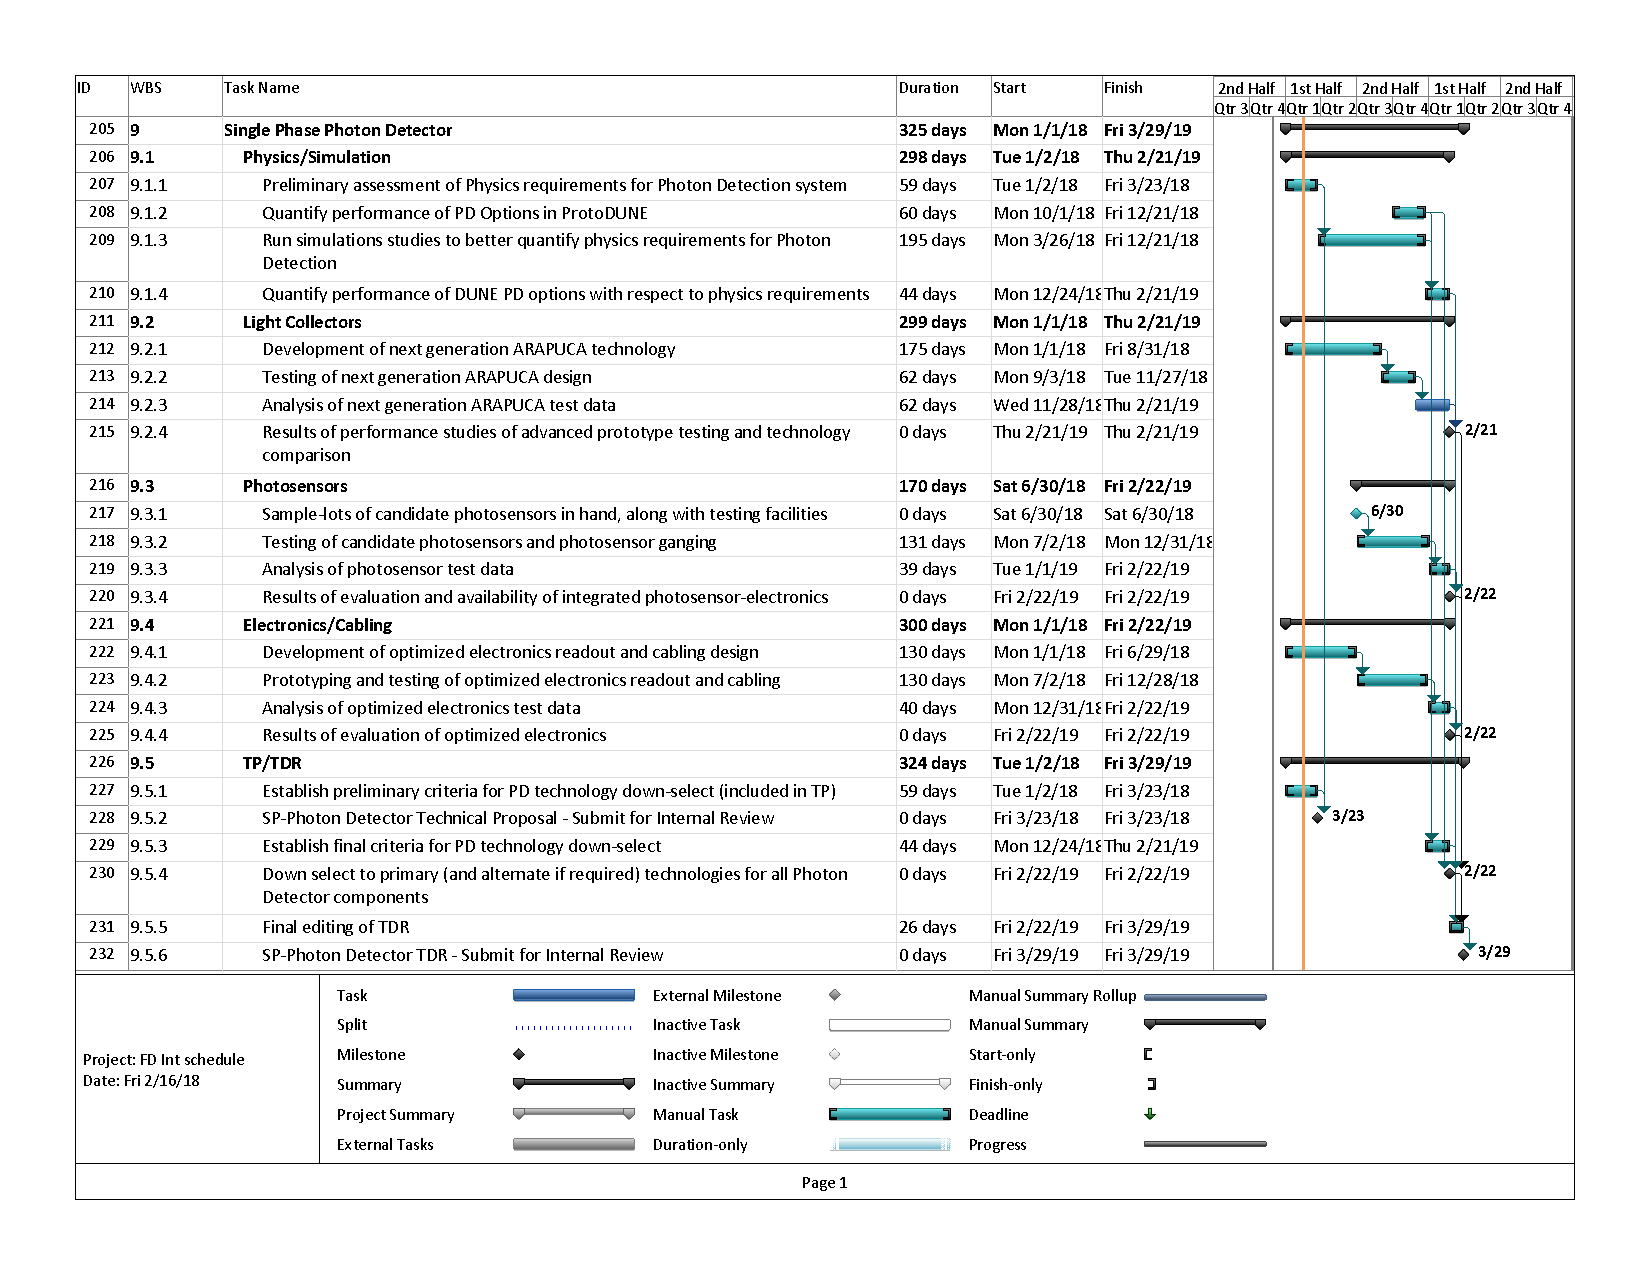
\includegraphics[width=1.0\columnwidth]{pds-sched-to-tdr.pdf}
\end{dunefigure}


\begin{dunetable}[Pre-Technical Design Report Key Milestones.]
{ll}
{fig:pds-pretdrkeymilestones}
{Pre-Technical Design Report Key Milestones.}
Milestone													&	Date	       \\ \toprowrule
Preliminary PD technology selection criteria determined				&	3/21/18	\\ \colhline
Results from final prototype light collector studies available			&	2/21/19	\\ \colhline
Final PD technology selection criteria available						&	2/21/19	\\ \colhline
Down-select to primary (and potential alternate) light collector technology	&	2/22/19	\\ \colhline
Submit initial TDR draft for internal review							&	3/29/19	\\ 
\end{dunetable}

High-level post-Technical Design Report milestones are listed in Table~\ref{fig:pds-posttdrkeymilestones}.

%LMM fixed detector -> Module below and 10 kt -> \SI{10}{kt}

\begin{dunetable}[Post-Technical Design Report Key Milestones.]
{ll}
{fig:pds-posttdrkeymilestones}
{Post-Technical Design Report Key Milestones.}
Milestone											&	Date	       \\ \toprowrule
PD pre-production review(s) complete					&	3/2020 	\\ \colhline
Initial PD module fabrication begins						&	9/2020	\\ \colhline
Final PD production review based on initial production QA		&	2/2021	\\ \colhline
First  PD modules delivered for installation				&	5/2021	\\ \colhline
Installation into \dwords{apa} begins							&	6/2021     \\ \colhline
PD fabrication complete (first \SI{10}{kt} module)			&	7/2023	\\ 
\end{dunetable}
